\section{可行方向与约束最优条件}
\label{sec:opt-con-optimality}

第~\ref{chap:optimization}章证明了：可微目标在开集内部的局部最小点处梯度为零。章首的预算例说明，这条结论在可行域边界上失效，因为边界点附近并非每个方向都能走。本节先只用可行域本身描述“哪些方向能走、沿这些方向目标不能下降”，得到不依赖约束写法的最优条件；再在约束函数满足适当正则条件时，把这一条件改写成约束梯度与乘子的代数关系，即KKT条件。

全章讨论的一般问题是
\begin{equation}
\label{eq:opt-con-problem}
  \min_{\bm x\in\mathbb R^d}f(\bm x)
  \quad\text{s.t.}\quad
  g_i(\bm x)\leq0\ (i=1,\dots,m),\qquad
  h_j(\bm x)=0\ (j=1,\dots,p),
\end{equation}
可行域记为$C=\{\bm x:g_i(\bm x)\leq0,\ h_j(\bm x)=0\}$，最优值$f^\star=\inf_{\bm x\in C}f(\bm x)$。对可行点$\bm x$，满足$g_i(\bm x)=0$的约束称为\term{活跃约束}（active constraint），其下标集合记为$I(\bm x)$；$g_i(\bm x)<0$的约束在$\bm x$附近不起限制作用。本章反复使用两个小例子。

\begin{example}[等式二次例]
\label{ex:opt-con-equality-qp}
最小化$f(\bm x)=\frac12(x_1^2+4x_2^2)$，约束$h(\bm x)=x_1+x_2-1=0$。目标的等值线是以原点为中心、横向拉长的椭圆，可行域是一条直线。
\end{example}

\begin{example}[预算分配例]
\label{ex:opt-con-budget}
给定$\tau>0$，最小化$f(\bm x)=\frac12\lVert\bm x-\bm c\rVert_2^2$，$\bm c=(2,1)^\top$，约束为$g_1(\bm x)=x_1+x_2-\tau\leq0$、$g_2(\bm x)=-x_1\leq0$、$g_3(\bm x)=-x_2\leq0$。可行域是三角形，最优点是$\bm c$在三角形上的最近点。
\end{example}

\subsection{可行方向与法向量}
\label{sec:opt-con-feasible-directions}

\paragraph{凸可行域上的变分不等式}
先设可行域$C$是凸集。站在可行点$\bm x$上，若另一点$\bm y\in C$，凸性保证线段$\bm x+t(\bm y-\bm x)$（$0\leq t\leq1$）都在$C$中，所以$\bm y-\bm x$是一个可以走的方向。局部最小点不允许沿任何这样的方向一阶下降，这给出下面的条件。

\begin{theorem}[凸可行域上的一阶条件]
\label{thm:opt-con-variational-inequality}
设$C\subseteq\mathbb R^d$非空凸，$f$在包含$C$的开集上可微。若$\bm x^\star$是$f$在$C$上的局部最小点，则
\begin{equation}
\label{eq:opt-con-vi}
  \langle\nabla f(\bm x^\star),\bm y-\bm x^\star\rangle\geq0\qquad\text{对所有}\ \bm y\in C.
\end{equation}
若$f$还在$C$上凸，则式~\eqref{eq:opt-con-vi}也是$\bm x^\star$为全局最小点的充分条件。
\end{theorem}

\begin{proof}
固定$\bm y\in C$，令$\varphi(t)=f(\bm x^\star+t(\bm y-\bm x^\star))$。$t\in[0,1]$时自变量在$C$中，且$t$足够小时它落在$\bm x^\star$的比较邻域内，所以$\varphi(t)\geq\varphi(0)$。于是右导数$\varphi'(0^+)=\langle\nabla f(\bm x^\star),\bm y-\bm x^\star\rangle\geq0$。若$f$凸，第~\ref{chap:optimization}章的一阶支撑下界给出$f(\bm y)\geq f(\bm x^\star)+\langle\nabla f(\bm x^\star),\bm y-\bm x^\star\rangle\geq f(\bm x^\star)$。
\end{proof}

式~\eqref{eq:opt-con-vi}称为一阶\term{变分不等式}（variational inequality）。它把“不能下降”写成对全部可行方向的检验：梯度可以不为零，但它必须与每个可行方向成不超过直角的夹角。把这个要求从梯度一侧改写到集合一侧，就得到法锥。

\begin{definition}[法锥]
\label{def:opt-con-normal-cone}
设$C$非空凸，$\bm x\in C$。集合
\[
  N_C(\bm x)=\{\bm v\in\mathbb R^d:\langle\bm v,\bm y-\bm x\rangle\leq0\ \text{对所有}\ \bm y\in C\}
\]
称为$C$在$\bm x$处的\term{法锥}（normal cone）。
\end{definition}

法锥中的向量与所有从$\bm x$出发的可行弦成钝角或直角，是“指向集合外侧”的方向；它对非负倍数和加法封闭，所以是凸锥。用这个记号，式~\eqref{eq:opt-con-vi}就是$-\nabla f(\bm x^\star)\in N_C(\bm x^\star)$：最优点处，下降最快的方向必须指向可行域外。

\paragraph{内点、光滑边界与角点}
法锥的大小随点的位置变化。图~\ref{fig:opt-con-normal-cone}在预算分配例（$\tau=2$）中改变理想分配$\bm c$，依次得到三种情形。若$\bm c=(0.6,0.8)^\top$在三角形内部，最近点就是$\bm c$本身；内点处每个方向都可行，法锥只有零向量，条件退回为$\nabla f(\bm x^\star)=\bm0$。若$\bm c=(2,1)^\top$，最近点$\bm x^\star=(3/2,1/2)^\top$位于斜边内部，法锥是斜边外法向$(1,1)^\top$的非负倍数；此时$-\nabla f(\bm x^\star)=\bm c-\bm x^\star=\frac12(1,1)^\top$正好在这条射线上。若$\bm c=(3,-1)^\top$，最近点是角点$(2,0)^\top$，法锥由两条边的外法向$(1,1)^\top$和$(0,-1)^\top$张成，$-\nabla f=(1,-1)^\top=1\cdot(1,1)^\top+2\cdot(0,-1)^\top$落在锥内。角点处可以直接验证式~\eqref{eq:opt-con-vi}：对三角形中任意$\bm y$，$\langle(1,-1)^\top,\bm y-(2,0)^\top\rangle=y_1-y_2-2\leq y_1+y_2-2\leq0$，其中用了$y_2\geq0$与$y_1+y_2\leq2$。

\begin{figure*}[!htbp]
  \centering
  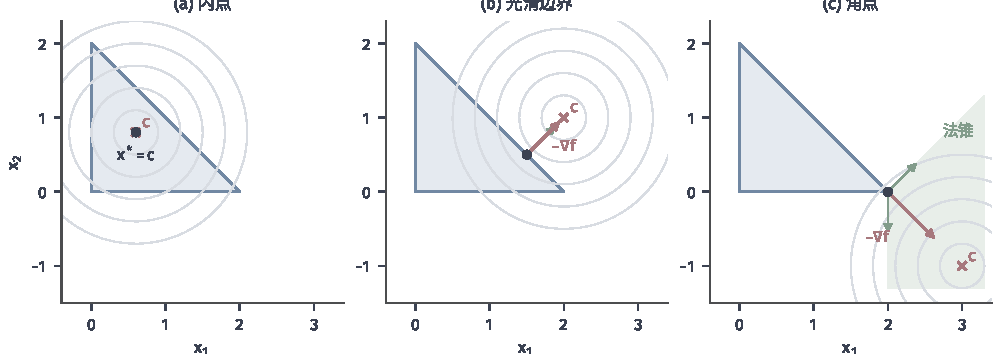
\includegraphics[width=169mm]{figures/03-optimization-evolution-and-signals/01-optimization/matplotlib/c5-normal-cone/figure.pdf}
  \caption{预算分配例（$\tau=2$）中最近点与法锥。浅蓝三角形为可行域，灰色圆为目标$\frac12\lVert\bm x-\bm c\rVert_2^2$的等值线，红叉为理想分配$\bm c$，黑点为最优点。(a) $\bm c$在内部，最优点处梯度为零；(b) 最优点在斜边上，红色箭头$-\nabla f$与绿色外法向同向；(c) 最优点在角点，绿色区域是两条外法向张成的法锥，$-\nabla f=(1,-1)^\top$落在其中。}
  \label{fig:opt-con-normal-cone}
\end{figure*}

三种情形说明，边界最优点的梯度通常不为零；判断最优性要看负梯度是否落在法锥中。光滑边界上的法锥是一条射线，角点处的法锥是一块锥形区域，因此角点能“容纳”更多方向的负梯度，这也是线性规划的解常落在顶点上的几何原因。

\paragraph{非线性约束：真实方向与线性化方向}
可行域由非线性约束给出时，它一般不是凸集，从$\bm x$出发的直线段可能立刻离开$C$。真实能走的方向要用可行点列来描述：若存在可行点$\bm x^{(k)}\to\bm x$和正数$t_k\downarrow0$，使$(\bm x^{(k)}-\bm x)/t_k\to\bm d$，就称$\bm d$属于$C$在$\bm x$处的\term{切锥}（contingent cone），记为$T_C(\bm x)$。它是闭锥，其中的方向可以由曲线或点列逼近，不必是直线段。

\begin{theorem}[切锥上的一阶必要条件]
\label{thm:opt-con-tangent-necessary}
设$f$在$\bm x^\star$附近可微，$\bm x^\star$是$f$在$C$上的局部最小点，则$\langle\nabla f(\bm x^\star),\bm d\rangle\geq0$对所有$\bm d\in T_C(\bm x^\star)$成立。
\end{theorem}

\begin{proof}
取$\bm d\in T_C(\bm x^\star)$及相应的$\bm x^{(k)}$、$t_k$。$k$足够大时$\bm x^{(k)}$落在比较邻域内，由Taylor展开，
\[
  0\leq\frac{f(\bm x^{(k)})-f(\bm x^\star)}{t_k}
  =\Bigl\langle\nabla f(\bm x^\star),\frac{\bm x^{(k)}-\bm x^\star}{t_k}\Bigr\rangle+\frac{o(\lVert\bm x^{(k)}-\bm x^\star\rVert_2)}{t_k}.
\]
由于$\lVert\bm x^{(k)}-\bm x^\star\rVert_2/t_k$有界，最后一项趋于零；令$k\to\infty$即得结论。
\end{proof}

切锥由可行域的几何决定，直接计算往往困难。实际可用的是约束函数的一阶近似：把活跃约束线性化，得到
\[
  L(\bm x)=\{\bm d:\langle\nabla h_j(\bm x),\bm d\rangle=0\ (\text{全部}\ j),\ \langle\nabla g_i(\bm x),\bm d\rangle\leq0\ (i\in I(\bm x))\},
\]
其中的方向称为\term{线性化可行方向}（linearized feasible direction）。真实方向总是线性化允许的：若$\bm d\in T_C(\bm x)$，对活跃的$g_i$有$0\geq g_i(\bm x^{(k)})-g_i(\bm x)=\langle\nabla g_i(\bm x),\bm x^{(k)}-\bm x\rangle+o(\lVert\bm x^{(k)}-\bm x\rVert_2)$，除以$t_k$再取极限得$\langle\nabla g_i(\bm x),\bm d\rangle\leq0$；等式约束同理得到等号。因此$T_C(\bm x)\subseteq L(\bm x)$。

反向包含可能不成立。图~\ref{fig:opt-con-cusp}中的可行域由$g_1(\bm x)=x_2-(1-x_1)^3\leq0$与$g_2(\bm x)=-x_2\leq0$给出，在$(1,0)^\top$处形成一个尖点。两条约束在该点都活跃，梯度分别为$(0,1)^\top$和$(0,-1)^\top$，线性化只要求$d_2=0$，于是$(1,0)^\top$和$(-1,0)^\top$都被允许；但当$x_1>1$时$(1-x_1)^3<0\leq x_2$，没有可行点，真实切锥只有$\{(-t,0)^\top:t\geq0\}$。线性化把一条不存在的方向当成了可行方向。取$f(\bm x)=-x_1$，点$(1,0)^\top$是全局最小点，满足定理~\ref{thm:opt-con-tangent-necessary}；可是线性化方向$(1,0)^\top$上$\langle\nabla f,\bm d\rangle=-1<0$，若只看线性化模型，会误以为还能下降。

\begin{figure}[!htbp]
  \centering
  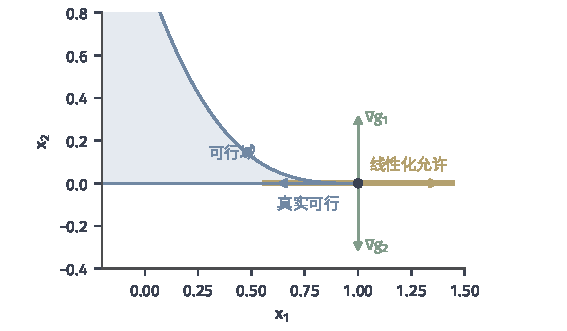
\includegraphics[width=96mm]{figures/03-optimization-evolution-and-signals/01-optimization/matplotlib/c5-cusp/figure.pdf}
  \caption{尖点处线性化方向多于真实方向。浅蓝区域为$x_2\leq(1-x_1)^3$且$x_2\geq0$的可行域，黑点为$(1,0)^\top$，绿色箭头为两条活跃约束的梯度。黄色线段表示线性化允许的方向$d_2=0$（左右两侧都允许），蓝色箭头是唯一真实可行的方向$(-1,0)^\top$。}
  \label{fig:opt-con-cusp}
\end{figure}

因此，从切锥上的必要条件过渡到只含约束梯度的条件，需要一个保证$T_C(\bm x)=L(\bm x)$的正则条件。下一小节先在这一条件下推出乘子，再用这个尖点说明条件缺失时乘子确实可能不存在。

\subsection{Lagrange乘子与KKT条件}
\label{sec:opt-con-kkt}

\paragraph{等式约束：梯度落在法向张成中}
图~\ref{fig:opt-con-tangency}画出等式二次例。沿约束直线移动时，目标值先降后升；在最优点，直线恰好与一条等值线相切。相切意味着梯度与直线的切向量$(1,-1)^\top$正交，即$\nabla f(\bm x^\star)$与约束的法向$\nabla h=(1,1)^\top$平行，可写成$\nabla f(\bm x^\star)+\nu\nabla h(\bm x^\star)=\bm0$，其中$\nu$是一个待定实数。这个系数称为\term{拉格朗日乘子}（Lagrange multiplier）。

\begin{figure}[!htbp]
  \centering
  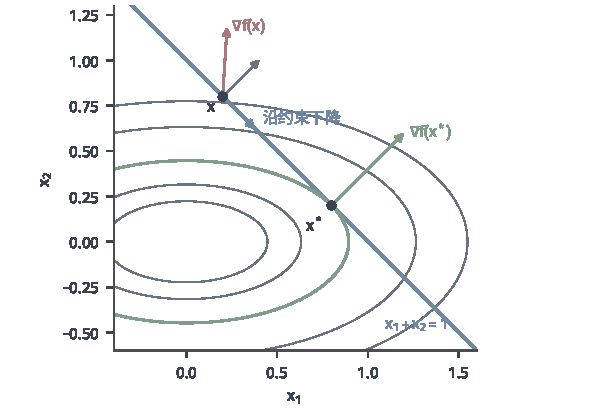
\includegraphics[width=100mm]{figures/03-optimization-evolution-and-signals/01-optimization/matplotlib/c5-tangency/figure.pdf}
  \caption{等式二次例的切点条件。灰色椭圆为$f(\bm x)=\frac12(x_1^2+4x_2^2)$的等值线，蓝线为约束$x_1+x_2=1$。在最优点$\bm x^\star=(4/5,1/5)^\top$，绿色等值线与约束线相切，梯度$(4/5,4/5)^\top$垂直于约束线。在非最优可行点$\bm x=(0.2,0.8)^\top$，红色梯度$(0.2,3.2)^\top$有沿约束线的分量，蓝色箭头所示的切向负分量仍能降低目标。}
  \label{fig:opt-con-tangency}
\end{figure}

在这个例子中，$\nabla f=(x_1,4x_2)^\top$，方程组$x_1+\nu=0$、$4x_2+\nu=0$、$x_1+x_2=1$给出$x_1=-\nu$、$x_2=-\nu/4$，代入约束得$-\frac54\nu=1$，所以$\nu^\star=-4/5$，$\bm x^\star=(4/5,1/5)^\top$，$f^\star=\frac12(16/25+4/25)=2/5$。对照非最优点$(0.2,0.8)^\top$：梯度$(0.2,3.2)^\top$在切向$(1,-1)^\top/\sqrt2$上的分量为$-3/\sqrt2\neq0$，沿$(1,-1)^\top$移动会降低目标，所以它不满足平行条件。

\paragraph{加入不等式：乘子的符号与互补松弛}
不等式约束只在活跃时限制移动，而且只限制向外的一侧。最优点处，负梯度应能写成活跃约束外法向的非负组合，这就是法锥的代数形式。以预算分配例（$\tau=2$）为例，最优点$\bm x^\star=(3/2,1/2)^\top$只使$g_1$活跃，$\nabla f(\bm x^\star)=(-1/2,-1/2)^\top$，取$\lambda_1=1/2$便有$\nabla f+\lambda_1\nabla g_1=\bm0$；未活跃的$g_2,g_3$取零乘子。若把$\bm c$换成$(3,-1)^\top$，最优点$(2,0)^\top$使$g_1,g_3$同时活跃，由$(-1,1)^\top+\lambda_1(1,1)^\top+\lambda_3(0,-1)^\top=\bm0$解出$\lambda_1=1$、$\lambda_3=2$，正是图~\ref{fig:opt-con-normal-cone}(c)中的分解。可以把$\lambda_i\nabla g_i$看成第$i$条约束施加的“反作用力”：目标推着点向$-\nabla f$方向走，活跃约束只能沿外法向往回推，且推力非负；最优点处各力平衡。

把等式与不等式合在一起，引入
\begin{equation}
\label{eq:opt-con-lagrangian}
  \mathcal L(\bm x,\bm\lambda,\bm\nu)=f(\bm x)+\sum_{i=1}^m\lambda_ig_i(\bm x)+\sum_{j=1}^p\nu_jh_j(\bm x),
\end{equation}
称为\term{拉格朗日函数}（Lagrangian）。“未活跃约束乘子为零”可以写成乘积$\lambda_ig_i(\bm x)=0$，这样就不必事先知道哪些约束活跃。

\begin{definition}[KKT条件]
\label{def:opt-con-kkt}
设$f,g_i,h_j$在$\bm x^\star$处可微。若存在$\bm\lambda^\star\in\mathbb R^m$、$\bm\nu^\star\in\mathbb R^p$，使
\begin{align*}
  &\text{驻点性：}&&\nabla f(\bm x^\star)+\textstyle\sum_i\lambda_i^\star\nabla g_i(\bm x^\star)+\sum_j\nu_j^\star\nabla h_j(\bm x^\star)=\bm0,\\
  &\text{原始可行性：}&&g_i(\bm x^\star)\leq0,\quad h_j(\bm x^\star)=0,\\
  &\text{对偶可行性：}&&\lambda_i^\star\geq0,\\
  &\text{互补松弛：}&&\lambda_i^\star g_i(\bm x^\star)=0\quad(i=1,\dots,m),
\end{align*}
就称$(\bm x^\star,\bm\lambda^\star,\bm\nu^\star)$满足\term{Karush--Kuhn--Tucker条件}（KKT conditions），简称KKT点。
\end{definition}

四组条件分工不同。驻点性就是$\nabla_{\bm x}\mathcal L=\bm0$，表达力的平衡；原始可行性保证候选满足约束；对偶可行性规定不等式乘子的方向；\term{互补松弛}（complementary slackness）规定只有活跃约束可以带正乘子。等式乘子没有符号限制，因为等式约束两侧都不能越过。互补松弛只说“乘子为正则约束活跃”，反过来不成立：预算分配例取$\tau=3$时，最优点$(2,1)^\top=\bm c$使预算约束恰好活跃，乘子却是零，因为目标本身已经不想越过预算线。

\paragraph{乘子存在所需的约束资格}
KKT条件是从局部最优推出来的必要条件，但这一推导需要条件。以下最常用的条件要求活跃约束的梯度彼此独立。

\begin{definition}[线性无关约束资格]
\label{def:opt-con-licq}
若全部$\nabla h_j(\bm x)$与活跃的$\nabla g_i(\bm x)$（$i\in I(\bm x)$）线性无关，就说可行点$\bm x$满足\term{线性无关约束资格}（linear independence constraint qualification，LICQ）。LICQ是一种\term{约束资格条件}（constraint qualification）。
\end{definition}

\begin{theorem}[LICQ下KKT条件的必要性]
\label{thm:opt-con-kkt-necessary}
设$f,g_i,h_j$在$\bm x^\star$的邻域内连续可微，$\bm x^\star$是问题~\eqref{eq:opt-con-problem}的局部最小点且满足LICQ，则存在唯一的$(\bm\lambda^\star,\bm\nu^\star)$使KKT条件成立。
\end{theorem}

\begin{proof}
记$\bm E$为以$\nabla h_j(\bm x^\star)^\top$为行的矩阵，$\bm B$为以活跃$\nabla g_i(\bm x^\star)^\top$为行的矩阵。

\emph{第一步：线性化方向都是真实方向。}LICQ说明$\begin{bmatrix}\bm E\\\bm B\end{bmatrix}$行满秩，故方程$\bm E\bar{\bm d}=\bm0$、$\bm B\bar{\bm d}=-\bm 1$有解$\bar{\bm d}$。先取严格方向$\bm d$，即$\bm E\bm d=\bm0$、$\bm B\bm d<\bm0$。考虑方程$\bm h(\bm x^\star+t\bm d+\bm E^\top\bm w)=\bm0$，未知量为$\bm w\in\mathbb R^p$；它在$(t,\bm w)=(0,\bm0)$成立，关于$\bm w$的Jacobian为$\bm E\bm E^\top$，由LICQ可逆。隐函数定理给出$t$附近的连续可微解$\bm w(t)$，$\bm w(0)=\bm0$，且$\bm w'(0)=-(\bm E\bm E^\top)^{-1}\bm E\bm d=\bm0$。曲线$\bm x(t)=\bm x^\star+t\bm d+\bm E^\top\bm w(t)$满足全部等式约束，且$\bm x(t)=\bm x^\star+t\bm d+o(t)$。对活跃的$g_i$，$g_i(\bm x(t))=t\langle\nabla g_i(\bm x^\star),\bm d\rangle+o(t)<0$；未活跃的$g_i$由连续性在$t$小时仍为负。所以$\bm x(t)$在小$t>0$时可行，$\bm d\in T_C(\bm x^\star)$。对一般$\bm d\in L(\bm x^\star)$，$\bm d+\varepsilon\bar{\bm d}$对每个$\varepsilon>0$都是严格方向，而切锥是闭集，令$\varepsilon\downarrow0$得$\bm d\in T_C(\bm x^\star)$。于是$T_C(\bm x^\star)=L(\bm x^\star)$。

\emph{第二步：由择一定理得到乘子。}由定理~\ref{thm:opt-con-tangent-necessary}，不存在$\bm d$使$\bm E\bm d=\bm0$、$\bm B\bm d\leq\bm0$且$\langle\nabla f(\bm x^\star),\bm d\rangle<0$。第~\ref{chap:opt-linear-programming}章的Farkas择一定理说：对矩阵$\bm M$和向量$\bm r$，系统$\bm M\bm u=\bm r,\ \bm u\geq\bm0$与系统$\bm M^\top\bm z\geq\bm0,\ \bm r^\top\bm z<0$恰有一个可行。取$\bm M=[\bm B^\top,\ \bm E^\top,\ -\bm E^\top]$、$\bm r=-\nabla f(\bm x^\star)$。若第二个系统有解$\bm z$，则$\bm d=-\bm z$满足$\bm B\bm d\leq\bm0$、$\bm E\bm d=\bm0$和$\langle\nabla f(\bm x^\star),\bm d\rangle=\bm r^\top\bm z<0$，与上面矛盾。所以第一个系统有解$\bm u=(\bm\lambda_I,\bm\nu^+,\bm\nu^-)\geq\bm0$，即$-\nabla f(\bm x^\star)=\bm B^\top\bm\lambda_I+\bm E^\top(\bm\nu^+-\bm\nu^-)$。令$\bm\nu^\star=\bm\nu^+-\bm\nu^-$，活跃乘子取$\bm\lambda_I$，未活跃乘子取零，四组KKT条件全部成立。乘子唯一，因为两组乘子之差会给出活跃梯度的一个非零线性组合等于零，与LICQ矛盾。
\end{proof}

回到尖点：在$(1,0)^\top$处两条活跃梯度$(0,1)^\top$与$(0,-1)^\top$线性相关，LICQ不成立。驻点方程$(-1,0)^\top+\lambda_1(0,1)^\top+\lambda_2(0,-1)^\top=\bm0$的第一个分量是$-1=0$，无解；最小点存在，乘子却不存在。更简单的例子是$\min x$、约束$x^2\leq0$：唯一可行点$0$是最小点，但$\nabla g(0)=0$，驻点方程$1+\lambda\cdot0=0$无解。LICQ只是约束资格的一种；凸问题中常用的Slater条件将在第~\ref{sec:opt-con-duality}节出现。

\paragraph{凸问题中KKT条件的充分性}
必要性回答“最优点是否一定有乘子”；反过来，已经拿到一组满足KKT条件的候选时，需要知道它是不是全局最优。凸结构给出肯定的回答，而且不需要任何约束资格。

\begin{theorem}[凸问题的KKT充分性]
\label{thm:opt-con-kkt-sufficient}
设$f$与各$g_i$是可微凸函数，各$h_j$是仿射函数。若$(\bm x^\star,\bm\lambda^\star,\bm\nu^\star)$满足KKT条件，则$\bm x^\star$是问题~\eqref{eq:opt-con-problem}的全局最小点。
\end{theorem}

\begin{proof}
固定乘子，函数$\bm x\mapsto\mathcal L(\bm x,\bm\lambda^\star,\bm\nu^\star)$是凸函数的非负组合加仿射函数，因而凸；驻点性说明它在$\bm x^\star$处梯度为零，所以$\bm x^\star$是它的全局最小点。对任意可行$\bm x$，$\lambda_i^\star g_i(\bm x)\leq0$、$h_j(\bm x)=0$，于是
\[
  f(\bm x)\geq\mathcal L(\bm x,\bm\lambda^\star,\bm\nu^\star)\geq\mathcal L(\bm x^\star,\bm\lambda^\star,\bm\nu^\star)=f(\bm x^\star),
\]
最后的等号用了互补松弛和$h_j(\bm x^\star)=0$。
\end{proof}

预算分配例的目标凸、约束仿射，所以前面算出的$\bm x^\star=(3/2,1/2)^\top$连同乘子$\lambda_1=1/2$已经证明了全局最优，无需再检查约束资格。非凸问题中KKT条件只是候选检验：在$[-1,1]$上最小化$f(x)=-x^2$，约束写成$x-1\leq0$、$-x-1\leq0$，点$x=0$不使任何约束活跃，驻点性$-2x=0$成立，乘子全取零便满足KKT条件，但它是全局最大点；真正的最小点$x=\pm1$也满足KKT条件，例如$x=1$处取$\lambda_1=2$。在非凸问题里，KKT条件筛掉的是明显不合格的点，留下的候选还需要比较目标值或用其他论证区分。
